\documentclass{tufte-handout}
\usepackage{amsmath,amsthm}

\input{vc.tex}

\usepackage{pgfplots}
\pgfplotsset{width=\textwidth}

\newtheorem{claim}{Claim}[section]
\title{\sf Exact Algorithm for Independent Set}
\date{\GITAuthorDate, rev. \GITAbrHash}
\author{}

\begin{document}
\maketitle

\section{Independent Set}
Consider an undirected unweighted graph $G=(V,E)$ and set $n=|V|$.
The Maximum Independent Set problem (MIS) is to find a subset $S$ of
the vertices of largest size such that no pair of different vertices
in $S$ are connected by an edge in $G$.
The size of the largest independent set in $G$ is denoted by
$\alpha(G)$.

MIS is NP-hard, but we will nevertheless implement algorithms that
compute $\alpha(G)$ for small instance graphs $G$ and argue both
empirically and theoretically about their running time.

\paragraph{Notation.}
For a subset $X\subseteq V$, we will by $G[X]$ denote the graph
\emph{induced} by $X$, the graph that remains if we keep only the
vertices in $X$ and the edges among them.
For a vertex $v$, we denote by $N[v]$ its \emph{closed neighborhood},
i.e. $v$ and all its neighbors.
We will slightly abuse set difference and union notation by using $-$
and $+$ instead.
$X+Y-Z$ for three sets $X,Y,Z$ are those elements that are in either
$X$ or $Y$ but not in $Z$.


\subsection{Algorithm $R_0$}

Consider the following simple recursive algorithm working on an input
graph $G=(V,E)$.
(Call it Algorithm~$R_0$):
\begin{enumerate}
\item
If the input graph is empty, return $0$;
\item
If the input graph $G$ has a vertex $v$ without any neighbors, return $1+R_0(G[V-v])$
\item Otherwise find a vertex $u$ of maximum degree (if there are
  several any will do) and return $\max(1+R_0(G[V-N[u]]),
  R_0(G[V-u]))$\sidenote{Observe once again that $N[u]$ is the
    \emph{closed neighborhood} of $u$, i.e., $u$ itself should also be
    removed.}.
\end{enumerate}

To see why algorithm $R_0$ correctly computes $\alpha(G)$, note that
if there is an isolated vertex $v$, a maximum size independent set
will always contain it (Row 2).
On the other hand, if there are no isolated vertices, we can pick a
vertex $u$ of maximum degree and branch on the two cases that $u$ is
in the maximum independent set (in which case we discard all vertices
adjacent to $u$ from $G$), or that $u$ is not in the maximum
independent set (Row 3).

\subsection{Inputs}

The data directory contains eleven random input instances of
increasing size. 
All input files are text files on the following format describing the
undirected graph $G=(V,E)$: First comes a positive integer $n$ giving
the number of vertices in the graph.
Next follow $n$ rows each containing $n$ $0/1$-entries describing the
so-called \emph{adjacency matrix} of the graph.
The $j$th integer at the $i$th row is a $1$ if and only if $ij\in E$.

\begin{marginfigure}
\begin{tabular}{lrr}
file & $|V|$ & $\alpha(G)$\\
 \texttt{g30.in} & 30 & 14\\
 \texttt{g40.in} & 40 & 16\\
 \texttt{g50.in} & 50 & 19\\
 \texttt{g60.in} & 60 & 20\\
 \texttt{g70.in} & 70 & 22\\
 \texttt{g80.in} & 80 & 24\\
 \texttt{g90.in} & 89 & 26\\
 \texttt{g100.in} & 100 & 27\\
 \texttt{g110.in} & 110 & 29\\
 \texttt{g120.in} & 120 & 30\\
 \texttt{g130.in} & 130 &  ? 
\end{tabular}
\end{marginfigure}



\subsection{Deliverables}

\begin{enumerate}
\item Implement algorithm $R_0$ and run it on the instances provided in
  data/g30.txt, data/g40.txt, ..., data/g60.txt.
  
  Count the number of recursive calls of $R_0$ for each instance and plot the
  logarithm of that number vs the instance vertex size. 
  
  What is the time complexity dependence on $n$?
  
  Use whatever programming language and libraries you want, but make
  sure that your code is not unnecessarily long.

  First implement the algorithm by making a new copy of the graph at
  each recursive call, just to make it as easy as possible to verify
  that the algorithm works as intended. Once you get this to work, you
  can pay attention to the problem of efficiently representing a graph
  through the recursion so that it is easy to remove (and add, see
  below) vertices to it by temporarily modifying the graph at hand.
   
  Attach a printout to the report or have it checked by your lab
  assistant.
\item Add the following line to algorithm $R_0$ after its first line
  checking for emptiness, and call the resulting algorithm $R_1$
  (replacing the recursive calls to $R_0$ by $R_1$):
 
 If $G$ has a vertex $v$ of degree $1$ return $1+R_1(G[V-N[v]])$.
 
 Argue the correctness of algorithm $R_1$, i.e., motivate why it always computes $\alpha(G)$.
 
 Implement algorithm $R_1$ and run it on the instances data/g30.in,
 data/g40.in, $\ldots$, data/g100.in.

  Count the number of recursive calls of R1 for each instance and plot the
  logarithm of that number vs the instance vertex size. 
  
  What is the time complexity dependence on $n$?

\item Add the following line to algorithm $R_1$ after its first line
  checking for emptiness, and call the resulting algorithm $R_2$
  (replacing the recursive calls to $R_1$ by $R_2$):
 
  If $G$ has a vertex $v$ with exactly two neighbors $u,w$, then if
  $uw\in E$ return $1+R_2(G[V-N[v]])$, else add a new vertex $z$ to
  the graph with edges to every neighbor of $u$ and $w$, except $v$,
  and return $1+R_2(G[V-N[v]+z)$.

  If $G$ doesn't have a vertex $v$ with exactly two neighbors, then we
  proceed just as in algorithm $R_1$.
 
 Argue the correctness of algorithm $R_2$, i.e.\ motivate why it always computes $\alpha(G)$.
 
 Implement algorithm $R_2$ and run it on the instances
  data/g30.in, data/g40.in, $\ldots$, data/g120.in.

  Count the number of recursive calls of $R_2$ for each instance and plot the
  logarithm of that number vs the instance vertex size. 
  
  What is the time complexity dependence on $n$?

\item Fill out the report on the next page; you can just use the
  \LaTeX\ code if you want.
\end{enumerate}

\newpage


\newpage
\section{Independent Set Lab Report}


by Alice Cooper and Bob Marley\sidenote{Complete the report by filling
  in your names and the parts marked $[\ldots]$.
  Remove the sidenotes in your final hand-in.}

\subsection{Correctness}
Algorithm R1 correctly computes $\alpha(G)$ because $[\ldots]$.\sidenote{Fill in the $[\dots]$ with an argument why R1 indeed computes the size of the maximum independent set. Use as little mathematical notation as necessary. A ``proof'' is whatever convinces me.}

Algorithm R1 will compute $\alpha(G)$ incorrectly if and only if the neighbour,
$n$, of a vertex of degree $1$, $v$, is in the $MIS$. The neighbour of $v$ has
$degree > 1$, otherwise one of them but not both may be in the $MIS$ and it
wont affect the result which one.

\begin{itemize}
	\item If the neighbour of $v$ is in the $MIS$, $v$ and at least one more
		vertex is not in the $MIS$.
	\item If $v$ is in the $MIS$ only its neighbour is not in the set and its
		neighbours neighbours may be.
\end{itemize}

Both cases will result in an identical graph with the exception that in case $v$
is in the $MIS$ at least one more vertex is still in the graph. Hence it must be
at least as good to include any vertex with $degree == 1$.

\noindent
Algorithm R2 correctly computes $\alpha(G)$ because $[\ldots]$.

\subsection{Empirical Running time}

\paragraph{Experiments.}
\sidenote{Plot the logarithm of the number of recursive calls for the
  three algorithms $R_0$, $R_1$, and $R_2$, in a combined image.
  
  Use whatever software you like to produce the image; the placeholder
  image on the left is constructed in the \LaTeX\ source, and should
  give you a feel of what the result could look like (with completely
  different values on the y-axis.)}

\medskip

\noindent
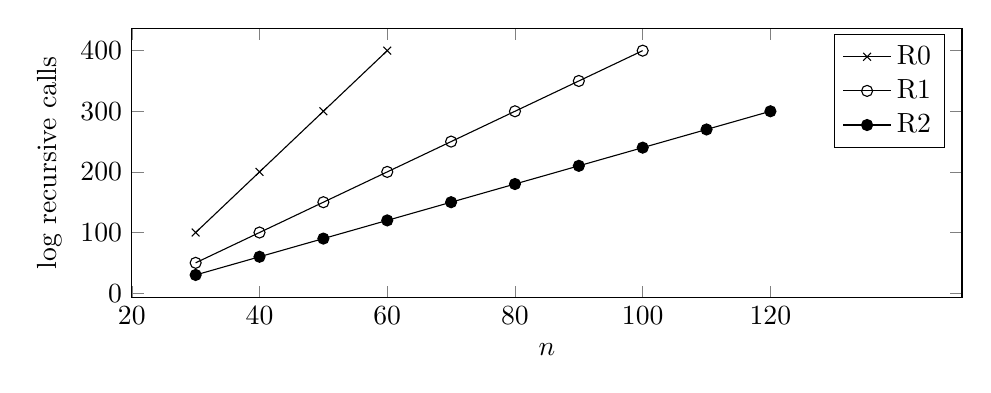
\begin{tikzpicture}
\begin{axis}[
  height= 5cm,
  xlabel=$n$,
  ylabel={log recursive calls},
  xmin = 20,  xmax = 150,
  xtick =       {20,40,60,80,100,120},
  xticklabels = { $20$, $40$, $60$, $80$, $100$, $120$},
  x tick label as interval = false,
  scaled ticks = false
]
    \addplot[color=black, mark=x] 
	coordinates {
	(30, 100)
	(40, 200)
	(50, 300)
	(60, 400)
    };
    \addlegendentry{R0}

    \addplot[color=black, mark=o] 
	coordinates {
	(30, 50)
	(40, 100)
	(50, 150)
	(60, 200)
	(70, 250)
	(80, 300)
	(90, 350)
	(100, 400)
    };
    \addlegendentry{R1}

    \addplot[color=black, mark=*] 
	coordinates {
	(30, 30)
	(40, 60)
	(50, 90)
	(60, 120)
	(70, 150)
	(80, 180)
	(90, 210)
	(100, 240)
	(110, 270)
	(120, 300)
    };
    \addlegendentry{R2}

\end{axis}
\end{tikzpicture}

The running times of algorithm~$R_0$, $R_1$, and $R_2$ appear to be
$[\ldots],[\ldots],$ and $[\ldots]$, respectively.\sidenote{Replace
  the $[\ldots]$ by a function of $n$ on the form $O(c^n)$.
  Use your measurements on the run time to estimate $c$ in the three
  cases.}.

\subsection{Theoretical Upper Bound}

Denote be $T_i(n)$ the worst runtime of algorithm Ri on \emph{any} graph on $n$ vertices.
Note that $T_i(n)$ is a non-decreasing function of $n$.
For $R_0$ we can conclude that
\begin{align*}
T_0(n) &\leq\max(T_0(n-1), T_0(n-1)+T_0(n-1-d_{\mbox{max}})) \\ &\leq T_0(n-1)+T_0(n-2)
\end{align*}
with $d_{\mbox{max}}$ the degree of the vertex we branch on. The hard part is the one when there are no isolated vertices, in which case the vertex $u$ we are branching on has at least one neighbor. 

For R1 we have that\sidenote{Derive similar recursive bounds on $T_1(n)$ and $T_2(n)$.}
 \[
 T_1(n)=[\ldots]
 \]

For R2 we have that
 \[
 T_2(n)=[\ldots]
 \]
\paragraph{Worst Case Upper Bound}
The running times of algorithm~$R_0$, $R_1$, and $R_2$ are in
$[\ldots],[\ldots],$ and $[\ldots]$, respectively.\sidenote{Replace
  the $[\ldots]$ by a function of $n$ on the form $O(c^n)$.
  Use the recursive bounds you've derived above.
  \emph{Hint: A recurrence of the form $T(n)\leq \sum_{i=1}^k
    a_iT(n-i)$ is called a linear homogeneous recurrence relation with
    constant coefficients.
    To solve it, you can set $T(n)\geq c^n$ where $c$ is the largest
    real root to the characteristic polynomial $x^k-\sum_{i=1}^k
    a_ix^{k-i}$}.}. \newpage

\section{Optional}
Add more ``algorithmic intelligence'' to the algorithm $R_2$ in order to tackle the instance in data/g130.in.
Try to make it run in less than 10,000,000 recursive calls. 

Suggestions for possible speed-ups:
\begin{itemize}
\item Is there some clever (branching) rule for vertices of degree 3?
\item Can we use the information of the largest found independent set so far, to reduce further computation time?
\item What if the graph gets disconnected?
\end{itemize}

\newpage
\section{ Perspective}

This lab establishes medium skills in recursive algorithms implementation,
and simple means to analyze their running time.

\bigskip

The algorithms investigated here can hardly be called ``advanced'', but the main message 
is that no one knows how to do significantly better with any other means.
Indeed, the strongest theoretical worst case run time bound for maximum independent set to date
is obtained by a computerized calculation on a huge set of branching reduction rules, just like the ones we've looked at here [Robson. Algorithms for maximum independent sets. Journal of Algorithms, 7(3):425--440, 1986]. For a much cleaner analysis with just a few rules, obtaining a comparative bound, see [Fomin, Grandoni, and Kratsch. A measure \& conquer approach for the analysis of exact algorithms, JACM 56 (5), article No. 25, 2009].


\end{document}
